% ============================================================================
%  CTSpinoPelvic1K - Medical Physics Dataset Article
%
%  REVTeX 4.2 with the AAPM substyle, which is what Medical Physics expects.
%  Overleaf: "Template for Medical Physics Journal" (RevTeX + aapm).
%
%  Article type: DATASET AND SOFTWARE ARTICLE (DS). AAPM policy PUB 3-C superseded the
%  Medical Physics Dataset Article policy (PUB 3-B) on 2026-05-16 and renamed the type.
%
%  THREE CONSTRAINTS SHAPE THIS FILE, all from the PUB 3-C policy:
%    1. Ten published pages.
%    2. NO HYPOTHESIS TESTING. Comprehensive descriptive analysis is REQUIRED and
%       visualization encouraged, but nothing may be framed as a result, tested for
%       significance, or offered as evidence for a mechanism.
%    3. The dataset DOI must exist before submission and be cited in the text.
%
%  See PLAN.md for the full requirements and the order of work.
% ============================================================================
\documentclass[aapm,mph,amsmath,amssymb,reprint]{revtex4-2}

\usepackage{graphicx}
\usepackage[table]{xcolor}
% Table 1 cells. \cellw is set inside the table from \linewidth so the nine class
% columns and the two text columns fill the text width exactly: no slack, so the
% filled cells of neighbouring columns touch and each header sits in its own column.
\newlength{\cellw}
\newcommand{\has}{\rule[-0.9ex]{\cellw}{3.1ex}}
\newcommand{\qual}{{\setlength{\fboxsep}{0pt}\setlength{\fboxrule}{0.5pt}\framebox[\cellw]{\rule[-0.6ex]{0pt}{2.4ex}}}}
\newcommand{\no}{\hspace{\cellw}}
\newcommand{\hd}[1]{\makebox[\cellw]{#1}}
\usepackage{booktabs}
\usepackage{siunitx}
\usepackage{tikz}
\usetikzlibrary{arrows.meta, positioning, fit, backgrounds, calc}
\usepackage[colorlinks=true,allcolors=blue]{hyperref}
% Continuous line numbering is a submission requirement. It comes from the
% `linenumbers' REVTeX class option above, NOT from the lineno package:
% lineno conflicts with amsmath and raises \prevdepth errors on every
% display equation.

% Reserve this on Zenodo BEFORE the final draft: a reserved DOI is quotable while the
% record is still private. Deleting that draft destroys the DOI and its files.
% The CONCEPT DOI, which always resolves to the current version. PUB 3-C added
% "Allow record versioning and file management" to the repository requirements, and a
% referee instructed to "verify existence/accessibility of material via supplied DOI"
% should land on the release this manuscript describes rather than a superseded one.
\newcommand{\datasetdoi}{10.5281/zenodo.22139642}
% The exact version this manuscript describes, for reproducibility.
\newcommand{\datasetversiondoi}{10.5281/zenodo.22293878}
\newcommand{\datasetversion}{v8}
% DOUBLE-ANONYMIZED REVIEW. \reviewtrue redacts the consortium's name and the self-citation.
% The DOIs are NOT redacted: PUB 3-C requires the dataset DOI to exist and be cited in the
% text, and a referee is instructed to verify it. Flip to \reviewfalse for camera-ready.
\newif\ifreview \reviewtrue
% The submission form wants the figure captions listed again after the references (the
% submitted preprint). The ten-page typeset check sets this false so they are counted once.
\newif\ifcaptionlist \captionlistfalse
\newcommand{\doiurl}[1]{\url{https://doi.org/#1}}
\newcommand{\consortium}{\ifreview a student research consortium\else OpenSpineConsortium\fi}

% Fit content to the text block WITHOUT enlarging it. \resizebox{\linewidth}{!}
% forces the width to match exactly, which scales small things UP -- inflating
% their fonts relative to the body text. This only ever shrinks.
\newsavebox{\fitbox}
\newcommand{\maxwidth}[1]{%
  \sbox{\fitbox}{#1}%
  \ifdim\wd\fitbox>\linewidth
    \resizebox{\linewidth}{!}{\usebox{\fitbox}}%
  \else
    \usebox{\fitbox}%
  \fi
}

% Fit content to what is left of a FLOAT PAGE once its caption has been set.
%
% MAXWIDTH CONSTRAINS ONE DIMENSION. Figure 1 is a tall flow chart and at full height it
% overran the page by 166pt -- to which LaTeX's answer is to set the graphic anyway and let
% the caption slide off the bottom edge. Nothing is reported as an overfull box, the figure
% looks correct, and its caption is simply not there.
%
% The caption is boxed FIRST so its height can be measured, because that height is not a
% constant: this file is compiled both preprint (single column, double spaced) and reprint
% (two column, single spaced), and a nine-line caption occupies very different amounts of
% page in the two. CAPTION is safe to build inside a box -- the counter steps and LABEL
% reads it as usual -- as long as the box is used in the same float.
\newsavebox{\capbox}
\newcommand{\fitfloat}[2]{% {graphic}{caption text, with its \label}
  \sbox{\capbox}{\parbox{\linewidth}{\caption{#2}}}%
  \sbox{\fitbox}{#1}%
  \ifdim \wd \fitbox>\linewidth
    \sbox{\fitbox}{\resizebox{\linewidth}{!}{\usebox{\fitbox}}}%
  \fi
  % resizebox keeps the aspect ratio, so fitting the width and then the height leaves the
  % smaller of the two scales -- which is the one that fits
  % ONE baseline of reserve, not three: on a float page the leftover is centered as white
  % space above and below, so every point held back here is a point of type size given up.
  \dimen0=\dimexpr \ht \fitbox+\dp \fitbox \relax
  \dimen2=\dimexpr \textheight-\ht \capbox-\dp \capbox-\baselineskip \relax
  \ifdim \dimen0>\dimen2
    \sbox{\fitbox}{\resizebox{!}{\dimen2}{\usebox{\fitbox}}}%
  \fi
  \usebox{\fitbox}\par \usebox{\capbox}%
}

% FLOAT PLACEMENT. With ten floats in a two-column article, LaTeX's defaults produce
% float-only pages and strand the text that should have shared them: before these were set,
% page 11 of the reprint carried 28 words and pages 3 and 9 carried about 300 each. The
% defaults are conservative -- a float may occupy at most 70% of the top of a page, and at
% least 20% of a page must be text -- which on a figure-dense article means a figure that
% could share a page with a column of prose instead takes one to itself.
%
% Loosening them costs nothing in correctness and recovers whole pages. \floatpagefraction
% raised to 0.75 also stops a float page being declared for a figure that leaves a quarter of
% the page blank.
\renewcommand{\topfraction}{0.92}
\renewcommand{\bottomfraction}{0.75}
\renewcommand{\textfraction}{0.06}
\renewcommand{\floatpagefraction}{0.78}
\renewcommand{\dbltopfraction}{0.92}
\renewcommand{\dblfloatpagefraction}{0.78}
\setcounter{topnumber}{3}
\setcounter{bottomnumber}{2}
\setcounter{totalnumber}{4}
\setcounter{dbltopnumber}{3}

\begin{document}
% Half of LaTeX's default separation under a two-column float: 20pt read as three
% blank lines between every figure* caption and the text beneath it.
\setlength{\dbltextfloatsep}{10pt plus 2pt minus 2pt}
\setlength{\textfloatsep}{10pt plus 2pt minus 2pt}

\title{CTSpinoPelvic1K: spine, pelvis, ribs and femora in one coordinate frame,
       annotated for lumbosacral transitional anatomy}

% DOUBLE-ANONYMIZED REVIEW: author names and affiliations live in title_page.tex and
% must NOT appear here. Restore this block only for the camera-ready version.
%\author{Gregory Schwing}
%\affiliation{Department of Surgery, Detroit Medical Center / Wayne State University, Detroit, Michigan, USA}
%\author{Ashley Schehr}
%\author{Annika Tekumulla}
%\author{Margret Khoushi}
%\author{Ryan Christian}
%\author{Dane Hubers}
%\author{Faris Mahjoub}
%\author{Hassan Saad}
%\author{Mia Sooch}
%\author{Sathya Siddapureddy}
%\author{Michael McLellan}
%\author{Jerick Kim}
%\affiliation{Wayne State University School of Medicine, Detroit, Michigan, USA}
\ifreview
\author{[Author names removed for double-anonymized review]}
\affiliation{[Affiliations removed for double-anonymized review]}
\else
\author{Gregory Schwing}\email{gregory.schwing@med.wayne.edu}
\affiliation{Department of Surgery, Detroit Medical Center and Wayne State University, Detroit, Michigan, USA}
\author{Ashley Schehr}
\author{Annika Tekumulla}
\author{Margret Khoushi}
\author{Ryan Christian}
\author{Dane Hubers}
\author{Faris Mahjoub}
\author{Hassan Saad}
\author{Mia Sooch}
\author{Sathya Siddapureddy}
\author{Michael McLellan}
\author{Jerick Kim}
\affiliation{School of Medicine, Wayne State University, Detroit, Michigan, USA}
\author{Miraziz Ismoilov}
\author{Nizar Alnabahneh}
\affiliation{Department of Radiology, Detroit Medical Center and Wayne State University, Detroit, Michigan, USA}
\fi
% [CO-AUTHOR] every author must supply their own conflict-of-interest statement;
% the declaration below covers all of them and only the first author has been asked.
% Affiliations were confirmed by the corresponding author: the annotators are School
% of Medicine, the two readers are Radiology.
%\author{Miraziz Ismoilov}
%\author{Nizar Alnabahneh}
%\affiliation{Department of Radiology, Detroit Medical Center / Wayne State University, Detroit, Michigan, USA}

\date{\today}

% ---------------------------------------------------------------------------
%  STRUCTURED ABSTRACT - four named sections, under 300 words.
% ---------------------------------------------------------------------------
\begin{abstract}
\textbf{Purpose:} A vertebra at the lumbosacral junction is named by counting. The gold
standard counts caudally from C2 on whole-spine imaging~\cite{lian2018}; however, a lumbar
case is planned on a lumbar study~\cite{acr2021,acrmri2023}, T12 to S1, without C2.
Abdominopelvic computed tomography (CT) holds that span plus the lowest ribs and pelvis,
standing in for the preoperative view. Where a
lumbosacral transitional vertebra (LSTV) alters the count, the local anatomy is ambiguous:
four rib-free vertebrae may be an L1 with a lumbar rib or an
L5 assimilated to the sacrum, and six may be a sixth lumbar vertebra, a T12 with aplastic
ribs, or a lumbarized S1~\cite{koninwalz2010}. CTSpinoPelvic1K asks whether local morphology
resolves that ambiguity without the count. Two public label sets already covered
this imaging, CTSpine1K's vertebrae and CTPelvic1K's pelvis, on the same colonography
patients, never joined; this release joins them on one series and annotates the bones
neither had. It provides 802 CT records with per-level ribs and femora, lumbar levels
anchored on the lowest rib-bearing vertebra and S1, and classes for L6, T13, a separate S1
and lumbar ribs, so anomalies are recorded as themselves.

\textbf{Acquisition and Validation Methods:} Records pair CTSpine1K~\cite{ctspine1k} and CTPelvic1K~\cite{ctpelvic1k} labels on each patient's bone-richest acquisition under a VerSe-native scheme. Validation: geometric invariants (802/802 pass); rib--vertebra incidence across 5{,}749 evaluable ribs (0.035\% offset); and spinopelvic measures matching published values.

\textbf{Data Format and Usage Notes:} NIfTI image/label pairs with patient-grouped LSTV-stratified five-fold splits and a reference loader; archived at \doiurl{\datasetdoi}.

\textbf{Potential Applications:} Classifying a vertebra from local features;
updating cadaveric morphometry;
spinopelvic assessment; opportunistic screening; and, absent a public
preoperative lumbar CT cohort, planning research (377 records prone).
\emph{Limitations:} thoracic ground truth is field-of-view limited; postural
angles recumbent; no held-out test set; ribs are triaged-review pseudolabels;
Castellvi grades are two-reader consensus.
\end{abstract}

\maketitle

% ---------------------------------------------------------------------------
\section{Introduction}

The spine commonly carries seven cervical, twelve thoracic and five lumbar vertebrae, and a
vertebra is identified by where it falls in that sequence. Transitional variants sit at the
two ends of the lumbar column, the thoracolumbar transitional vertebra (TLTV) above and the
lumbosacral transitional vertebra (LSTV) below, and they disturb identification in two
ways at once. They change what the border vertebra and its ribs \emph{look like}: a
thoracolumbar border vertebra may carry a full rib, a hypoplastic stump, or none at all, and
a lumbosacral one may be partly or completely assimilated to the sacrum
(\emph{sacralization}), with an anteriorly wedged body, a reduced disc beneath it and
hypoplastic facet joints, or conversely separated from it (\emph{lumbarization}), with a
squared body, lumbar-type facets and a full-height disc~\cite{koninwalz2010}. They also
change \emph{how many} vertebrae each region contains: eleven or thirteen thoracic, four or
six lumbar.

Either change alone would be tractable. Together they make it difficult to state definitively
what any vertebra at these borders \emph{is}. Four rib-free vertebrae above the sacrum may mean
an L1 bearing a lumbar rib or an L5 assimilated to it; six may mean a true sixth lumbar
vertebra, a T12 whose ribs are aplastic, or an S1 lumbarized away from the sacrum. Each
set yields the same count, and the morphology that would separate the readings is not
decisive to a human reader in every case. Whether it differs enough for a learned classifier to separate them, or at
least to assign each reading a probability, is the question this release is built to
support. Absent that, what remains is the count itself: the gold standard for numeration in
transitional anatomy is whole-spine imaging, counting caudally from C2~\cite{lian2018},
which fixes how many vertebrae and how many rib pairs the column holds, and no
spine-limited acquisition can supply either count. LSTV is common,
reported between 4\% and 30\% depending on definition, and wrong-level surgery is its most
serious consequence.

Existing public collections cannot address this, and size is not the reason
(Table~\ref{tab:priorart}). Spine datasets omit the pelvis; pelvic datasets do not number the
vertebrae; TotalSegmentator, the whole-body scheme, has no class for a sixth lumbar vertebra
or for a rib on a lumbar vertebra; and VerSe, the one collection with an L6 class, stops at
the sacrum and carries no ribs. No public collection can therefore record a six-lumbar spine
together with both of its borders, however good the segmentation, and a segmenter trained on
them inherits the gap: faced with an enumeration anomaly it must shift the whole column by a
level or absorb a vertebra into its neighbor. The size of that problem has now been measured
on CT, where prior labeling methods assigned every vertebra correctly in 77\% of subjects and
an anomaly-aware extension of SPINEPS~\cite{spineps2025} raised that to
99\%~\cite{veridah2026}. Its weights label L6 and T13 on CT, but its 1{,}536 training scans are in-house and unreleased: the capability exists as weights, not as data. 

The intraoperative side of the problem has prior art of its own. LevelCheck registers the
intraoperative radiograph to the preoperative CT and projects the CT's vertebral labels onto
it, localizing the target level in a limited field of view to within a few percent of cases
in clinical use~\cite{otake2012,lo2015,desilva2016}. The labels it projects are placed by
hand on the CT, by a skilled operator and verified by the surgeon~\cite{otake2012}: the
method assumes a correctly labeled CT and does not supply one. Automating that step, and
getting it right precisely where the anatomy is anomalous, is what a dataset carrying the
classes those anomalies produce is for.

CTSpinoPelvic1K places the spine, pelvis, ribs and femora in one coordinate frame and gives
a class to each structure an enumeration anomaly produces: a sixth lumbar vertebra, and a
rib borne by a lumbar vertebra. A scheme without those classes lacks a class vocabulary
expressive enough to describe anatomic anomalies.

The project began as a surgeon's question: whether a vertebra can be named from the
anatomy in front of the reader, on the images a lumbar case is actually planned on: by
guideline those are lumbar studies~\cite{acr2021,nass2013,acrmri2023}, T12 to S1, and whole-spine
coverage is reserved for trauma with an identified injury~\cite{tqip2018} and for deformity
radiographs. The cohort suits that question: an abdominopelvic CT runs from the diaphragm to the pelvic
floor, so it holds the T12-to-S1 span of the planning study together with the lowest ribs
and the whole pelvis, and it lacks C2 exactly as that study does. Every record
comes from one prospective trial protocol, ACRIN 6664~\cite{colonog,tcia}: 802 patients aged
50 and over, scanned supine and prone on multidetector CT at 15 centers, on five scanner
vendors and nine models, with manufacturer, model and reconstruction kernel recorded per
record. To our knowledge it is the largest spine-and-pelvis annotated CT cohort acquired
under a single protocol; the comparators pool several collections (CTSpine1K four,
CTPelvic1K seven), are multi-site by design (VerSe), or are routine clinical scans under
many protocols (TotalSegmentator). With the protocol held fixed, scanner effects on a
model become measurable rather than confounded. The price is the field of view: abdominal,
so only the lowest thoracic levels are present and C2 never is (Sec.~\ref{sec:applications}).

The gap was in plain sight. CTPelvic1K~\cite{ctpelvic1k} and CTSpine1K~\cite{ctspine1k},
released months apart by an overlapping author group, each annotated the COLONOG
collection under radiologist supervision, one the pelvis and the other the vertebrae, on the
same patients, and no one joined them, although the join needs no new imaging and no new
radiologist. It is not a file merge: every patient was scanned prone and supine and neither
source recorded which series it drew on, so each annotation had to be traced back to its
own series (Sec.~\ref{sec:sources}). Done once, that crosswalk yields a spine-and-pelvis
frame at 802 patients for the cost of the crosswalk, and the bones neither set had, ribs, femora,
S1 and hardware, could then be annotated against it rather than from scratch. Two of the
most-used public bone annotation sets were halves of one dataset; this release is the whole.

\emph{Where the material is.} Everything described here is \datasetversion{} of one archived
dataset, \doiurl{\datasetversiondoi}; cite the concept DOI \doiurl{\datasetdoi}, which
resolves to the current version (Sec.~\ref{sec:format}).

\subsection{Vertebra labeling when the scan cannot settle the count}

\emph{The limitation, stated plainly.} No scan in this corpus contains C2, so the
conventional count cannot be performed: a property of abdominal imaging, not of the
annotation. A thirteenth thoracic vertebra and a lumbar rib on L1 are the same object under two
names, and either removes one rib-free vertebra from the count between the two borders of the
lumbar spine, the last rib-bearing vertebra and the sacrum, whereas an aplastic twelfth rib
adds one. A \emph{stump rib} (a hypoplastic twelfth rib, a cardinal indicator of a
thoracolumbar transitional vertebra) is still a rib: it leaves the count unchanged, and only
its length records the anomaly. Without C2, a count of four therefore cannot separate a
thirteenth thoracic vertebra from a lumbar rib, and a count of six cannot separate an
aplastic twelfth rib from a sixth lumbar vertebra.

\emph{What the release does in addition.} Every vertebra carries the identifier its
radiologist-sourced annotation assigned, corrected where the source was wrong; those labels
are the ground truth. Alongside them, every released measurement is also expressed against
the two landmarks present in essentially every abdominal scan, the sacrum below and the
lowest rib-bearing vertebra above, so that the measurement is positional rather than
nominal: a vertebra by how many rib-free vertebrae
separate it from the sacrum, a lowest rib by its length as a fraction of the rib above it, a
transverse process by its span and its distance from the ala. None of these changes according
to whether a reader would have said L5 or S1, so cases that disagree about the name remain
comparable, and where the junction is in view the count is determined and the two
descriptions agree.

\emph{But the vertebrae themselves are known to differ.} Counting is not the only route to
an identity. Level-specific morphometry is long established: pedicle width and height change
systematically from the thoracic to the lumbar spine,\cite{zindrick1987} vertebral body,
endplate and canal dimensions differ by level,\cite{panjabi1991,panjabi1992,benzel2015} and
the transverse process and the iliolumbar ligament mark the last lumbar vertebra
independently of any count.\cite{hughes2006,koninwalz2010} If those differences hold at the
boundary itself, the phenotype is decidable from the vertebra in front of the reader without
any global count. On this corpus it does hold:
separating T12 from L1 on shape alone, with each patient's own size divided out and
cross-validation grouped by case, gives an area under the curve of 0.990 and 97.3\%
accuracy over 1485 vertebrae. Size is removed because raw millimeters separate thoracic
from lumbar trivially and teach nothing about the junction, where the two are nearly the
same size.

That is reported as a property of the released measurements rather than as a method: the
information needed to settle these variants is present locally.

% ---------------------------------------------------------------------------


\begin{table*}[t]
\caption{Public CT collections at the lumbosacral junction. Black, class present; outlined,
graded only to exclude it~\cite{versedata2021}.}
\label{tab:priorart}
\begin{ruledtabular}
% nine class columns sized to fill the text width with the two text columns: no slack,
% so neighbouring filled cells touch and every header sits inside its own column
\setlength{\cellw}{\dimexpr(\linewidth-50mm)/9\relax}%
\begin{tabular}{@{}l@{}r@{\hspace{4mm}}l@{}}
Collection & Scans & \hd{Count}\hd{L6}\hd{Sacrum}\hd{S1}\hd{Pelvis}\hd{Ribs}\hd{L.\,rib}\hd{Femora}\hd{Grade} \\ \colrule
CTSpine1K~\cite{ctspine1k} & 1{,}005 & \has\has\no\no\no\no\no\no\no \\
CTPelvic1K~\cite{ctpelvic1k} & 1{,}184 & \no\no\has\no\has\no\no\no\no \\
VerSe~\cite{verse2021} & 374 & \has\has\no\no\no\no\no\no\qual \\
RibSeg~v2~\cite{ribsegv2} & 660 & \no\no\no\no\no\has\no\no\no \\
TotalSegmentator~\cite{totalsegmentator} & 1{,}204 & \has\no\has\has\has\has\no\has\no \\
\textbf{CTSpinoPelvic1K} & 802 & \has\has\has\has\has\has\has\has\has \\
\end{tabular}
\end{ruledtabular}
\end{table*}

\section{Acquisition and Validation Methods}

\begin{figure}[t]
\centering
% Single-spaced inside the chart whatever the document does: in the double-spaced preprint
% the boxes inherited the stretch, the float grew past the page, and every later figure
% queued behind it to the end of the paper.
\linespread{1}\selectfont
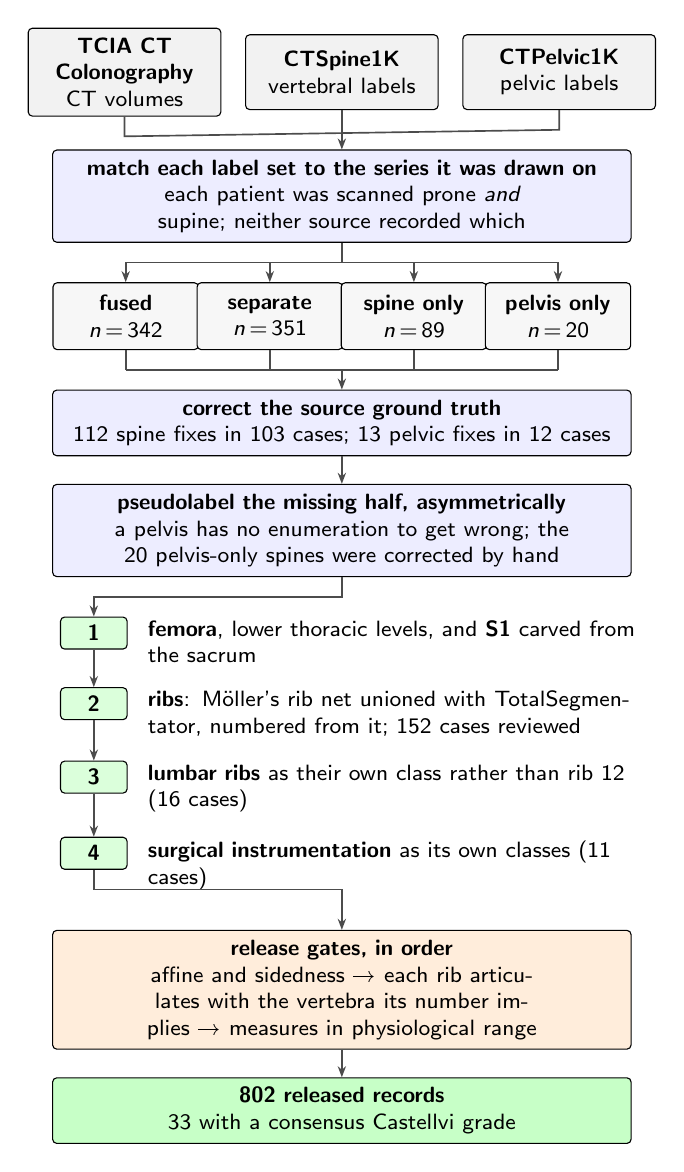
\begin{tikzpicture}[
  % absolute 8 pt: the boxes are sized in millimetres, so the type must not follow the
  % document size (\footnotesize is 10 pt in the preprint and wrapped every box)
  x=1mm, y=1mm, font=\sffamily\fontsize{8}{9.6}\selectfont, node distance=3.5mm,
  bx/.style={draw, rounded corners=1.5pt, align=center, text width=#1, inner sep=3.5pt},
  src/.style={bx=22mm, fill=black!5, minimum height=9.5mm},
  proc/.style={bx=71mm, fill=blue!7},
  rec/.style={bx=16mm, fill=black!3, minimum height=8.5mm},
  ver/.style={bx=6mm, fill=green!14, inner ysep=3pt},
  det/.style={align=left, text width=62mm, inner sep=0pt},
  gate/.style={bx=71mm, fill=orange!14},
  fin/.style={bx=71mm, fill=green!22},
  ar/.style={-{Stealth[length=4pt]}, semithick, black!70},
  ln/.style={semithick, black!70},
]
% sources
\node[src] (spine) at (0, 0) {\textbf{CTSpine1K}\\vertebral labels};
\node[src, left=3mm of spine]  (tcia)   {\textbf{TCIA CT Colonography}\\CT volumes};
\node[src, right=3mm of spine] (pelvic) {\textbf{CTPelvic1K}\\pelvic labels};
\node[proc, below=5mm of spine] (cross) {\textbf{match each label set to the series it was drawn on}\\
  each patient was scanned prone \emph{and} supine; neither source recorded which};
\draw[ln] (tcia.south) -- ($(tcia.south)+(0,-2.5mm)$) -- ($(pelvic.south)+(0,-2.5mm)$) -- (pelvic.south);
\draw[ar] (spine.south) -- (cross.north);
% record types, on a bus
\node[rec, anchor=north] (fused) at ($(cross.south)+(-27.45mm,-5mm)$) {\textbf{fused}\\\textit{n}\,=\,342};
\node[rec, anchor=north] (sep)   at ($(cross.south)+(-9.15mm,-5mm)$)  {\textbf{separate}\\\textit{n}\,=\,351};
\node[rec, anchor=north] (sonly) at ($(cross.south)+(9.15mm,-5mm)$)   {\mbox{\textbf{spine only}}\\\textit{n}\,=\,89};
\node[rec, anchor=north] (ponly) at ($(cross.south)+(27.45mm,-5mm)$)  {\mbox{\textbf{pelvis only}}\\\textit{n}\,=\,20};
\draw[ln] (cross.south) -- ($(cross.south)+(0,-2.5mm)$);
\draw[ln] ($(fused.north)+(0,2.5mm)$) -- ($(ponly.north)+(0,2.5mm)$);
\foreach \n in {fused,sep,sonly,ponly} \draw[ar] ($(\n.north)+(0,2.5mm)$) -- (\n.north);
% corrections and pseudolabels
\node[proc, anchor=north] (fix) at ($(cross.south |- fused.south)+(0,-5mm)$) {\textbf{correct the source ground truth}\\
  112 spine fixes in 103 cases; 13 pelvic fixes in 12 cases};
\foreach \n in {fused,sep,sonly,ponly} \draw[ln] (\n.south) -- ($(\n.south)+(0,-2.5mm)$);
\draw[ln] ($(fused.south)+(0,-2.5mm)$) -- ($(ponly.south)+(0,-2.5mm)$);
\draw[ar] ($(fix.north)+(0,2.5mm)$) -- (fix.north);
\node[proc, below=of fix] (dense) {\textbf{pseudolabel the missing half, asymmetrically}\\
  a pelvis has no enumeration to get wrong; the 20 pelvis-only spines were corrected by hand};
\draw[ar] (fix.south) -- (dense.north);
% versions
\node[ver, anchor=north west] (v3) at ($(dense.south west)+(1mm,-5mm)$) {\textbf{1}};
\node[det, anchor=north west] (d3) at ($(v3.north east)+(2.5mm,-0.5mm)$) {\textbf{femora}, lower thoracic levels, and \textbf{S1} carved from the sacrum};
\node[ver, anchor=north west] (v4) at ($(v3.south west |- d3.south)+(0,-3mm)$) {\textbf{2}};
\node[det, anchor=north west] (d4) at ($(v4.north east)+(2.5mm,-0.5mm)$) {\textbf{ribs}: M\"oller's rib net unioned with TotalSegmentator, numbered from it; 152 cases reviewed};
\node[ver, anchor=north west] (v5) at ($(v4.south west |- d4.south)+(0,-3mm)$) {\textbf{3}};
\node[det, anchor=north west] (d5) at ($(v5.north east)+(2.5mm,-0.5mm)$) {\textbf{lumbar ribs} as their own class rather than rib~12 (16 cases)};
\node[ver, anchor=north west] (v6) at ($(v5.south west |- d5.south)+(0,-3mm)$) {\textbf{4}};
\node[det, anchor=north west] (d6) at ($(v6.north east)+(2.5mm,-0.5mm)$) {\textbf{surgical instrumentation} as its own classes (11 cases)};
\draw[ar] (dense.south) -- ($(dense.south)+(0,-2.5mm)$) -| (v3.north);
\draw[ar] (v3.south) -- (v4.north); \draw[ar] (v4.south) -- (v5.north); \draw[ar] (v5.south) -- (v6.north);
% gates and release
\node[gate, anchor=north] (qc) at ($(dense.south |- d6.south)+(0,-5mm)$) {\textbf{release gates, in order}\\
  affine and sidedness \textrightarrow\ each rib articulates with the vertebra its number implies
  \textrightarrow\ measures in physiological range};
\draw[ar] (v6.south) -- ($(v6.south)+(0,-2.5mm)$) -| (qc.north);
\node[fin, below=of qc] (rel) {\textbf{802 released records}\\33 with a consensus Castellvi grade};
\draw[ar] (qc.south) -- (rel.north);
\end{tikzpicture}
\caption{How the dataset was built. $n$ counts scans, or corrections, at each step.}
\label{fig:pipeline}
\end{figure}

\subsection{Sources, and why a crosswalk was necessary}\label{sec:sources}

Both sources draw part of their imaging from the TCIA CT colonography
collection~\cite{colonog,tcia}. CTSpine1K's 1{,}005 volumes come from four
collections and CTPelvic1K's 1{,}184 from seven; COLONOG is the only collection common to
both and the only one acquired under a single protocol, so this release is its COLONOG
subset: 782 patients with a CTSpine1K vertebral annotation and 20 with a CTPelvic1K pelvic
annotation only, 802 in all. Neither source released the mapping from an annotation to the
specific CT series it was drawn on.

That mapping matters because every patient in CT~COLONOGRAPHY was scanned \emph{twice},
prone and supine, and an annotation carries a patient identifier and nothing finer. Turning
a patient from supine to prone alters lumbar lordosis and the alignment of each segment
against the next, so outlines drawn on one series are the wrong \emph{shape} for the other
and no rigid realignment recovers them. The crosswalk (Fig.~\ref{fig:pipeline}) therefore
resolves each annotation to a patient and then, within that patient's volumes, to the series
whose bone \emph{agrees} with it: candidates are thresholded at bone attenuation and scored
by overlap with the mask.

\subsection{Fused and split records}

CTSpine1K and CTPelvic1K each annotated a patient independently, so their labels are not guaranteed to come from the same CT series (Fig.~\ref{fig:pipeline}). This turned out to matter for 351 patients, nearly half the cohort: the two collections had labeled different acquisitions of the same person, one prone and one supine, with neither recording which. Because posture changes spinal alignment, a spine label from one acquisition cannot simply be paired with a pelvic label from the other. These 351 records are released but held out of any analysis that assumes a single posture; two labeled postures of one patient are a resource for studying alignment, not a defect. 

\subsection{Densification, and why it is asymmetric}

A corpus in which half the records lack a pelvis is not a spinopelvic dataset, so the
missing structures were pseudolabeled, asymmetrically (Fig.~\ref{fig:pipeline}). Pelvis
onto spine-only records is the safe direction: the sacrum and innominate bones carry no
enumeration to get wrong, and quality is reported as held-out performance on the
\emph{pelvic\_only} records, withheld from training for that purpose. The reverse direction
carries the whole problem this dataset addresses, since a pseudolabeled spine must commit to
a count and on a transitional vertebra commits to the commoner reading; those 20 records were
corrected by hand, tractable at that scale.

\subsection{Ribs}

No public rib annotation covers this cohort, and the two available automatic sources fail
in complementary ways.

Möller's binary rib network~\cite{moller2026} reports high accuracy, and its authors show
that stump ribs can be classified from a partial field of view; that result concerns the
morphological features computed on a rib once segmented. On this corpus the segmentation
itself failed on ribs that were \emph{partially outside} the field of view: a rib crossing
the boundary of an abdominal acquisition was liable to be missed altogether rather than
segmented to the edge. Its authors do not report this: their evaluation excluded subjects
whose last rib was not visible, so it is recorded here as an observation from this cohort. In a colonography cohort the lower ribs are routinely clipped, and
those are the ribs the count depends on.

TotalSegmentator~\cite{totalsegmentator} does segment clipped ribs and supplies the
per-rib numbering that a binary network cannot. Its characteristic failure is at the other
end of the bone: the most medial portion of the rib (roughly the last tenth to sixth
approaching the costovertebral joint) is frequently absent. A rib truncated at its
medial end never reaches the vertebra it articulates with, so the rib--vertebra incidence
check (the quality-control gate on the rib class labels, which matches each rib to the
vertebra its number implies) has nothing to test.

The two were therefore unioned (Fig.~\ref{fig:pipeline}), TotalSegmentator supplying the
numbering and the medial-clipped cases, Möller the detection where its output is more
complete.

The result is a pseudolabel whose review was triaged rather than exhaustive. A label-based
rule flagged every record in which one rib
bone carried more than one identifier, or in which a rib failed to reach the vertebra it
articulates with, since a single bone carrying two numbers is a numbering error by construction,
whatever the anatomy. The rule selected 152 records; 148 were reviewed and corrected, and four
were not and are identified in the release. Reviewers were medical students working through
\consortium~\cite{osc2026}, trained against a written labeling protocol, with every
correction recorded against the annotator who made it. Records passing the rule were not
individually inspected, so the layer only guarantees freedom from the failure modes the rule detects, no more. The residual rib--vertebra offsets reported in
Sec.~\ref{sec:validation} are the independent check on what the rule missed.

\subsection{Label scheme and counting anchors}

The scheme is VerSe-native: vertebrae keep their VerSe identifiers (C1--C7 = 1--7,
T1--T12 = 8--19, L1--L6 = 20--25, sacrum 26, coccyx 27, T13 = 28), and every non-VerSe
structure takes a fixed identifier above that range: S1 carved from the sacrum (29), hips
(30--31), femora (32--33), ribs (34--45 left, 46--57 right), lumbar ribs (58--59) and
surgical hardware (60--66). The space is contiguous; there is no class for a thirteenth
rib, because a rib on the vertebra below T12 is recorded as a lumbar rib whatever that
vertebra is called.

Two anchors make the count decidable, and Fig.~\ref{fig:anchors} shows both: the lowest
rib-bearing vertebra above, \textbf{S1} carved from the sacrum below. Each earns its place
by what it supports rather than by being an endpoint. S1 supplies the sacral endplate
landmark that sacral slope and pelvic incidence are measured from, and with both brackets
present L5 and L6 are distinguishable where a spine-limited view alone would not be.

\emph{How S1 is cut.} The sacrum's outer boundary is the source annotation and is never
altered; S1 is the cranial part of that same bone, separated by a plane. The plane's normal
is the sacrum's own cranio-caudal axis, made orthogonal to a left--right axis
measured directly rather than assumed, so as to remove the patient's rotation within the scanner. That rotation is not
negligible: median 4.5\textdegree{}, maximum 16.1\textdegree{}, and 508 of 801 records above
3\textdegree{}. The cut preserves the sub-division volume of the preceding release,
changing the orientation of the S1/S2 boundary and not how much sacrum is called S1;
per-record geometry ships with the archive.

Neither anchor is novel on its own: TotalSegmentator~\cite{totalsegmentator} carries a
separate S1 class and per-level ribs, and VerSe~\cite{verse2021} carries L6, whose
identifier this release keeps, so its L6 \emph{is} VerSe's.

\textbf{A rib on a lumbar body receives its own class}, and this is the one class here with
no published counterpart. A lumbar rib and a stump rib are the same object under two counts,
so assigning it a number would commit the label to one reading of an enumeration anomaly. A
scheme that numbers every rib 1--12 has nowhere to put a thirteenth: the annotator must
either call it rib~12, asserting the vertebra beneath it is thoracic, the very question at
issue, or discard it. TotalSegmentator carries ribs 1--12 per side and no such class, and
VerSe's T13 is a vertebra rather than a rib. This scheme can record both: VerSe's T13 (28)
for a thoracic-type thirteenth vertebra with a true rib, and 58/59 for a lumbar-type body
bearing a rudimentary one, so either reading is recorded as itself. No record here carries
a T13; the sixteen lumbar-rib cases were read as lumbar-type bodies. Where a border vertebra
could not be settled by its readers the label stands as read, and reclassifying those
records with a classifier trained on local vertebral morphology
(Sec.~\ref{sec:applications}) is the intended path for a later release.

\begin{figure*}[t]
\centering

\includegraphics[width=\linewidth,keepaspectratio]{figures/fig_anchors.pdf}
\caption{The two anchors, from the released labels. Red, lowest rib-bearing vertebra and
its rib; blue, S1; yellow, the rib-free vertebrae between. (b) and (c) both count four: in (b) the last rib is on L1, in (c) on T12 with L5 assimilated to the sacrum.}
\label{fig:anchors}
\end{figure*}

Figure~\ref{fig:anchors} shows why the interval is the primitive and the label is derived.
Among the records with four rib-free vertebrae, some reach that count from above, through a rib on L1, and some from below, through an L5 assimilated to the sacrum; the count alone cannot tell them apart, and the release can because the rib and the S1 boundary are both labeled.

Sixteen records carry a lumbar rib: thirteen bilateral and three unilateral, all on the
right, a count too small to support any statement about side preference.

Eighteen records carry an L6. Seventeen of them carry a consensus Castellvi grade;
the eighteenth was not graded. The source transitional label, an independent field, reads
lumbarization in fourteen, sacralization in two and semi-sacralization in one, and is
unremarkable in the ungraded record: a spine can carry six lumbar-type vertebrae and still
be read as a sacralization, depending on where the reader started the count.

Both counts, and the manifest fields that report them (\texttt{has\_l6},
\texttt{has\_lumbar\_rib}, \texttt{n\_lumbar\_labels}, \texttt{lumbar\_rib\_side}), are
computed from the released label volumes by counting identifiers 25 and 58--59.

\subsection{Computational tools}

\emph{Access.} Every step is performed by open-source code archived with the dataset,
together with the reference loader, the label scheme and the quality-control scripts that
generated the tables in this manuscript.

\emph{Versions and parameters.} Segmentation of femora, the sacral sub-division and the
per-level rib numbering used TotalSegmentator~\cite{totalsegmentator} (\texttt{total} task,
release 2.x) on a single graphics processing unit. The binary rib network is
M\"oller's~\cite{moller2026} released weights, applied through the nnU-Net v2
framework~\cite{nnunet}. The pelvic completion for records whose pelvis was absent used a
five-fold nnU-Net v2 ensemble, applied out-of-fold: each record is completed by the fold that
never trained on it, so no record is completed by a model that has seen it. The five fold
checkpoints, with their nnU-Net plans and dataset descriptor, are released alongside the
data (\ifreview the repository URL identifies the authors; it is on the title page and will be
restored here for the camera-ready version\else\url{https://huggingface.co/OpenSpineConsortium/spinopelvic-seg-checkpoints}\fi). Image handling
throughout used NiBabel and SciPy; no image is resampled or reoriented when a label is
written, so every label shares its image's grid and affine exactly.

\emph{Generative artificial intelligence.} A large language model (Claude, Anthropic)
assisted with drafting and editing the manuscript text and with writing the analysis and
figure code, all under author review. It was not used to generate, annotate or interpret
imaging data; every number reported here is computed by the released code from the
released volumes.

\subsection{Validation}
\label{sec:validation}


Validation runs in three layers, and the geometric layer runs first: a measurement
made on an inconsistent corpus returns a number that looks as finished as a correct one.

\emph{Geometric invariants.} Every case is checked for label geometry agreeing with its CT
in shape, affine and voxel spacing; for identifiers within the published scheme; for a
non-empty label; and for sided structures falling on the correct sides, with the left--right
axis read from the affine rather than assumed. The check exists because a renumbering pass
once wrote a reoriented array under a canonical affine and transposed a label away from its
image, a failure invisible downstream.

The check compares \emph{each sided pair separately}: testing the ribs alone passed all
802 records while four carried \texttt{left\_hip} on the patient's right, and pooling all
sided structures into one test still missed one of those four, because a large
correctly-sided structure masks a smaller transposed one. A gate that passes everything is
not evidence of a clean corpus until it has been shown capable of failing.

\emph{Rib--vertebra incidence.} Each rib is matched to its nearest vertebra and compared
against the vertebra its number implies. Of 11{,}548 ribs, 5{,}788 are not evaluable
because the expected vertebra lies outside the field of view and 11 have no vertebra within
the anchor distance; of the 5{,}749 evaluable, 5{,}747 match, two (0.035\%) are offset by one
level, and no case is misnumbered. The denominator is stated because quoting the two
offsets against all 11{,}548 ribs would halve the rate by counting ribs the check never
examined. Both offsets are field-of-view truncations on individually characterized cases,
one at $+1$ level and one at $-1$, reported rather than suppressed.

The same check carries an invariant that reads as a null result. Of the 5{,}749 evaluable
ribs, \emph{zero} are assigned to a lumbar vertebra, not because no lumbar ribs exist,
since 16 records carry one, but because such a rib takes class 58 or 59 and never enters the
numbered set the test examines. A numbered rib landing on a lumbar vertebra would be a
counting error of exactly the kind this dataset exists to expose.

\emph{Agreement with published values.} Derived spinopelvic measures are compared against
Vialle \emph{et al.}~\cite{vialle2005} (Table~\ref{tab:spinopelvic}). Pelvic incidence is
the strongest of these checks because it is a morphological property of the pelvis rather
than a posture, and so is directly comparable to a standing reference cohort.

\subsection{Castellvi typing}

Every record whose vertebral count departs from five carries a Castellvi
grade~\cite{castellvi1984} in the released manifest: 33 cases, typed I--IV with the $a$/$b$
unilateral--bilateral qualifier. The grade and the count are \emph{different axes}: grade
IIIb occurs here at rib-free counts of four, five and
six alike, and seven of the 33 graded cases carry a normal count of five.

Two radiology resident physicians graded every case independently and resolved their six
disagreements by consensus; both reads and the consensus are in the manifest. The distinction
the readers disagreed on, type II (articulation) against type III (bony
fusion)~\cite{koninwalz2010}, is the one that matters clinically: four of the six
disagreements were III against II.

\begin{table*}[t]
\caption{Derived measures against a standing reference ($n=260$)~\cite{vialle2005}; this
cohort is supine.}
\label{tab:spinopelvic}
\begin{ruledtabular}
\maxwidth{%
\begin{tabular}{lcc}
Measure & This dataset (supine) & Reference (standing) \\ \colrule
Pelvic incidence & 54.7\si{\degree} & 54.7 $\pm$ 10.6 \\
Pelvic tilt & 17.3\si{\degree} & 13 $\pm$ 6 \\
Sacral slope & 36.9\si{\degree} & 41.0 $\pm$ 8.4 \\
Lumbar lordosis (supine) & 52.7\si{\degree} & 43 $\pm$ 11.2 (standing) \\
PI $-$ LL mismatch & 2.6\si{\degree} & centered near 0 \\
\end{tabular}
}
\end{ruledtabular}
\end{table*}

% ---------------------------------------------------------------------------
\subsection{Surgical hardware, and why a threshold is not enough}
\label{sec:hardware}

Metal is trivial to detect and hard to interpret, and the difference matters here because
\textbf{an iatrogenic fusion is indistinguishable from a congenital one to a distance
measurement}: a cage-bridged interspace reads as ``no gap'' exactly as a fused transitional
vertebra does.

\paragraph{Detection over-calls by a factor of five.} A 2500\,HU threshold inside a shell
around the labeled skeleton flags 52\ of the 802\ records. One of the two radiology
resident physicians read all 52\ and confirmed 11, rejecting 41\ (79\%) as contrast,
calcification and reconstruction artefact. Attenuation does not separate the two groups
(both saturate); site and volume do, every confirmed implant at 2,586\,mm$^3$ or above and
every rejection at 1,768\,mm$^3$ or below.

\paragraph{The subtype block had to be extended.} Identifiers 60--63 name spinal
instrumentation (generic, cage, screw-and-rod, plate) and cannot describe what this cohort
holds, so \textbf{64 arthroplasty}, \textbf{65 sacroiliac screw} and \textbf{66
osteosynthesis} were added: osteosynthesis holds parts of one bone together where
arthroplasty replaces a joint, and a shape rule calls a femoral stem a rod. The confirmed
cases are eight arthroplasties, one osteosynthesis, one sacroiliac fixation and one pair of
interbody cages (Fig.~\ref{fig:hardware}).

\paragraph{Metal outranks bone, and that is a subtraction.} In every confirmed case the
implant was already inside a bone label, so naming it reclaims 1,538,852\ voxels rather
than adding them. In eight of these cases the femoral head that pelvic incidence and tilt are
measured from is an implant.

\begin{figure*}[t]
\centering

\includegraphics[width=\linewidth,keepaspectratio]{figures/fig_hardware.pdf}
\caption{Instrumentation in the release, one exemplar each, drawn through bone. (a) Hip
arthroplasty, 64, $n=8$. (b) Femoral-neck screws, 66, $n=1$. (c) Sacroiliac screws, 65,
$n=1$. (d) Interbody cages, 61, $n=1$. Bar, 5\,cm.}
\label{fig:hardware}
\end{figure*}

% ---------------------------------------------------------------------------
\section{Data Format and Usage Notes}\label{sec:format}

Each record is a gzipped NIfTI image/label pair sharing an identical $4\times4$ affine,
canonicalized to PIR, requiring no resampling. Masks are NIfTI rather than DICOM, which is what volumetric segmentation tooling expects.

Splits are patient-grouped and LSTV-stratified five-fold, frozen and shipped with the data
as \texttt{splits\_5fold.json}. The five validation folds partition all 802 records, so the
release provides cross-validation and \emph{not} a held-out test set; users reporting a
single held-out number should carve one out and state which records it holds.

Stratification is on the transitional subtype rather than a binary LSTV flag: every
validation fold carries three sacralization and three lumbarization records. With 15 of
each across 802 that is the most stratification can guarantee, and it is why a fold-level
metric on the rare classes carries an error bar far wider than its own decimal places.

\begin{table*}[t]
\caption{\label{tab:completeness}Data types and metadata, and the records populating
each, from the released manifest.}
\begin{ruledtabular}
\begin{tabular}{lrr}
Field & Records & Available \\
\hline
Identifier, image path, label path, configuration, match type & 802 & 100.0\% \\
Patient position, tube potential, section thickness, kernel & 802 & 100.0\% \\
Transitional label and class & 802 & 100.0\% \\
Spine and pelvic annotation origin & 802 & 100.0\% \\
Instrumentation and partial-annotation flags & 802 & 100.0\% \\
Image/label alignment check & 802 & 100.0\% \\
Spine series identifier; bone-fraction check & 782 & 97.5\% \\
Scanner manufacturer and model & 768 & 95.8\% \\
Sex & 749 & 93.4\% \\
Age & 709 & 88.4\% \\
Pelvic series identifier & 713 & 88.9\% \\
Castellvi grade (consensus of two readers) & 33 & 4.1\% \\
\end{tabular}
\end{ruledtabular}
\end{table*}

Table~\ref{tab:completeness} lists the key data types and metadata against the fraction of
records for which each is populated.

The archive of record is Zenodo (\doiurl{\datasetdoi}). Code and documentation are on GitHub at
the tagged release commit; any model-hub copy is a convenience mirror, not the archive.

% ---------------------------------------------------------------------------
\section{Descriptive Analysis}
\label{sec:descriptive}

\begin{figure*}[t]
\centering

\includegraphics[width=\linewidth,keepaspectratio]{figures/fig_countfree.pdf}
\caption{Count-free measures. (a) Vertebrae between the lowest rib and the sacrum.
(b) Lowest rib length over the rib above. (c) Lowest lumbar transverse span against its gap
to the ala; transitional labels marked.}
\label{fig:countfree}
\end{figure*}

The cohort is a colorectal cancer screening population of 802 records. 738 are recorded
female (393) or male (345); 11 carry DICOM's \emph{other} value and 53 no sex field. Age is present for 709 (median 59, range 50--89).
All 802 are counted in totals; the eleven records outside the female/male dichotomy are
excluded from sex-stratified measures rather than folded into ``unrecorded''. The lower
age bound is the screening guideline, not a selection applied here.

\emph{Count-free measures} (Fig.~\ref{fig:countfree}). Five rib-free vertebrae above the
sacrum is typical; four and six are where transitional anatomy sits, and which of the two
is present does not by itself determine what to call it. The lowest-rib length ratio is bimodal.

\emph{Level gradients and spinopelvic measures} (Fig.~\ref{fig:validation}). Vertebral
dimensions increase caudally; pelvic incidence does not vary with age while pelvic tilt
does, the signature of a pelvis retroverting as a spine ages.

% Left full-width deliberately: narrowing this one to a column saved no page and cost
% legibility in a five-panel figure. The hardware figure was worth narrowing; this is not.
\begin{figure*}[t]
\centering

\includegraphics[width=\linewidth,keepaspectratio]{figures/fig_validation.pdf}
\caption{Spinopelvic measures against standing reference bands (mean $\pm$
SD)~\cite{vialle2005}.}
\label{fig:validation}
\end{figure*}



\emph{Opportunistic measures.} Every scan carries a
vertebral bone density measurement at no additional dose.\cite{pickhardt2013} L1 trabecular attenuation is
reported at the published standard site.

% ---------------------------------------------------------------------------
\section{Potential Applications and Limitations}\label{sec:applications}

The principal use is the \emph{spinopelvic interface}. Spine and pelvis carry
radiologist-sourced annotation on one coordinate frame in 802 records, making sacral
morphology measurable against the lumbar column rather than in isolation: the sacral
endplate and its slope, the alar corridors constraining S2-alar-iliac and iliac screw
trajectories, and the L5--S1 geometry a lumbosacral fusion must cross. Pelvic incidence is
derived from the segmented sacrum and femoral heads rather than from landmarks placed on a
radiograph, so it is reproducible from the labels themselves.

The transitional layer serves that use rather than competing with it: no trajectory can be
planned across a junction whose segments cannot be named.

\emph{A proxy for the preoperative view.} No public preoperative lumbar CT cohort exists that we know of, and VerSe, the largest public spine CT collection, lacks the sacrum and pelvis (Table~\ref{tab:priorart}). This release is therefore the closest available stand-in for the view a lumbar case is planned on: the T12-to-S1 span with the lowest ribs and the pelvis; 377 of 802 records acquired prone, the position of posterior lumbar surgery; and classes for the anomalies that make level identification fail. It is a screening population at colonography dose, reconstructed with standard soft-tissue kernels rather than the bone kernel of a surgical CT, and not a surgical series: it supports method
development for level identification and instrumentation geometry, not validation of a
planning decision.

\subsection{Three uses the released measurements support}

\emph{Naming a level from its own geometry.} Wrong-level spine surgery runs at roughly one in
3{,}110 spinal procedures, and the cause most often cited is the transitional anatomy this
cohort was assembled around.\cite{epstein2021} Per-level body height, canal width,
endplate width, transverse-process span and wedge ratio are released for T11--L5 across all
802 records, and because the labels were assigned against the twelfth rib rather than by
enumeration, a model trained on them is not learning the convention that fails.

\begin{figure*}[t]
\centering

\includegraphics[width=\linewidth,keepaspectratio]{figures/fig_levelatlas.pdf}
\caption{Morphometry by level: median, interquartile range, 5th--95th percentile, $n$ at
right. (a) Body height. (b) Endplate width. (c) Canal. (d) Pedicle width. (e) Disc height.
(f) Trabecular attenuation.}
\label{fig:levelatlas}
\end{figure*}

\emph{Reference morphometry with its spread.} The values a surgeon consults for vertebral
body height, canal dimensions and pedicle width come from cadaveric series of a few dozen
specimens, plotted as single values with no indication of spread.\cite{benzel2015} They
cannot tell a reader whether the patient in front of them is unusual, because they never
show what usual looks like. The same measures are given here from 802 records with the
distribution attached (Fig.~\ref{fig:levelatlas}), reproducing two properties of the
classical figures (body height crosses over, dorsal exceeding ventral at T11--T12 and
reversing by L4--L5, and pedicle width widens steeply into the lower lumbar spine) and
adding the width of each distribution, which is the part needed to judge an individual.

\emph{Patient-specific models.} Planning is moving toward patient-specific biomechanical
models rather than population norms.\cite{fea2026} Such a model needs spine, pelvis and
femoral heads in one frame, which is this release's construction; in 351 patients two
postures give a within-patient change in alignment against which a predicted postural
response can be checked.

Its limitations are stated at the level of detail a reader would
need to catch them independently.

\begin{figure}[t]
\centering

\includegraphics[width=\linewidth,keepaspectratio]{figures/fig_fov.pdf}
\caption{Records carrying each vertebral level, cranial to caudal. Counts per identifier
in Table~S1.}
\label{fig:fov}
\end{figure}

\emph{Coverage.} Thoracic ground truth is field-of-view limited (Fig.~\ref{fig:fov}) and
does not extend to T1.
Postural angles are supine; pelvic incidence is not postural and needs no such caveat. The
cohort is a colorectal screening population aged 50 and over, so its distributions should
not be read as representative of a surgical one.



\emph{Strength of the labels varies by structure, and the release does not average over
that.} Vertebral labels derive from radiologist-supervised source annotations, corrected
where those sources were wrong. Pelvic labels on records that lacked one are
pseudolabeled. The rib layer is a pseudolabel whose human review was triaged by an
automated rule rather than exhaustive, so its guarantee is the absence of the failure modes
that rule detects. Transitional labels derive from two independent sources and are not
uniformly adjudicated, which is precisely why the measures reported here are count-free,
and the Castellvi grades are a consensus of two radiology resident physicians.
S1 is carved from the sacrum by an automatic estimate of the S1--S2 boundary, and in
100 records that estimate is implausible: it makes S1 more than half the sacrum's height or
less than fifteen percent of it. Those records are flagged in the released quality-control
table and should be excluded from any measurement that depends on the sacral endplate.

\emph{Structures are not universally present.} Sacrum, hips and femora are present in all 802 records; one record carries no S1, one lacks T12, and nine lack an L5 identifier, because the structure lies outside the field of view or, for L5, because the lowest lumbar segment is labeled L6 or incorporated into the sacrum. Users needing the caudal anchor should filter on it explicitly.

\section{Discussion}

\emph{Comparison with related material.} Against the collections in
Table~\ref{tab:priorart}, the contribution is the crosswalk placing spine and pelvis on the
same series, together with classes for the anatomy an enumeration anomaly actually produces. VerSe~\cite{verse2021,versedata2021} comes closest in intent, enriching for transitional anatomy and grading by Castellvi, but it does not segment the sacrum, so the structure a grade describes has no mask; this release segments it, as L6 or as a separately carved S1. Adding a sacrum to VerSe would not have supplied the pelvis, the femora or a prone acquisition, and here both label sets already existed: the join cost a crosswalk, not an annotation campaign.  What this release adds over TotalSegmentator~\cite{totalsegmentator} is not more anatomy per scan but the classes an anomaly needs to be recorded accurately. 

\emph{Limitations.} The cohort comes from one acquisition protocol of a colorectal-screening population aged 50 and over, so how well it generalizes to a pathologic population is untested. The rib layer's human review was triaged by an automated rule rather than performed on every bone, so it guarantees only the absence of the failure modes that rule detects. 

\emph{Future directions.} Imaging beyond this protocol, and the C2 anchor it cannot supply, are the natural next additions; applying the released weights to VerSe would add the S1 anchor and the anomaly classes to a bone-kernel spine collection, and VerSe's vertebra labels would score that transfer.

\section{Conclusion}

CTSpinoPelvic1K places spine, pelvis, per-level ribs and femora on one coordinate frame in
802 records, and gives the anatomy that makes lumbar numbering ambiguous a class of its own
rather than recording it as something it is not. Because both counting anchors are explicit,
a level can be identified from a field of view that cannot support the conventional count
downward from C2, which is every record here.

\section*{Data Availability}
The release described here is \datasetversion{}, permanently archived at
\doiurl{\datasetversiondoi}; the concept DOI \doiurl{\datasetdoi} resolves to the
current version.
The archive carries the loader, the label scheme, the quality-control tables and the
analysis code under an open-source licence. \ifreview The repository URL identifies the authors; it
is on the title page and will be restored here for the camera-ready version.\else Code:
\url{https://github.com/OpenSpineConsortium/CTSpinoPelvic1K}; convenience mirror:
\url{https://huggingface.co/datasets/OpenSpineConsortium/CTSpinoPelvic1K}.\fi

\section*{Acknowledgements}
% The guidelines want the COI statement below an Acknowledgements section, and the
% acknowledgements themselves on the title page for double-anonymized review.
Acknowledgements are given on the title page, per the journal's double-anonymized review
policy. This work received no funding.

\section*{Conflict of Interest}
The authors have no relevant conflicts of interest to disclose.

\section*{Ethics}
% The determination arrived on 2 September 2026. It is stated here without the institution
% or the HPR number, both of which would defeat the double-anonymization; those are on the
% title page.
This work uses publicly available, de-identified imaging and annotations derived from it.
The authors' institutional review board determined that it is not human participant
research under 45 CFR 46 and requires no oversight.

\begin{thebibliography}{20}
% GENERATED, DO NOT HAND-EDIT. Produced from ctspinopelvic1k.bib through the journal's
% medphy.bst and pasted here as the template README instructs, because REVTeX's aapm
% substyle emits its own \bibdata and a second \bibliography command makes bibtex refuse
% the run. To change a reference, edit the .bib and re-run:
%     pdflatex bibtest && bibtex bibtest && python inline_bbl.py
%
% Every entry was verified against the publisher record, Crossref or arXiv in September
% 2026. Verification corrected three errors that had survived in the hand-typed list:
%   * osc2026    first author is Schehr, not Schwing
%   * moller2026 the title belonged to a different paper; it is now the published
%                preprint, which also settles the citable form the co-author was to choose
%   * ctspine1k  the preprint has appeared in Mach. Learn. Biomed. Imaging
% A trade-press item was removed rather than published unverified: its host returns 403 to
% automated retrieval, so the attribution rested on search snippets and not on the page. The
% claim it supported now cites a peer-reviewed review of the same subject.
%
% \sloppy in the reference list only: a news-article URL with no hyphens to break on
% overflows the two-column measure, and loosening inter-word spacing among the references
% is a smaller cost than a line running into the margin.
\sloppy

\bibitem{lian2018}
J.~Lian, N.~Levine, and W.~Cho,
\newblock A review of lumbosacral transitional vertebrae and associated vertebral numeration,
\newblock Eur. Spine J. {\bf 27}, 995--1004 (2018),
\newblock doi:10.1007/s00586-018-5554-8.

\bibitem{acr2021}
Expert Panel on Neurological Imaging, T.~A. Hutchins, M.~Peckham, et~al.,
\newblock {ACR} {Appropriateness} {Criteria} low back pain: 2021 update,
\newblock J. Am. Coll. Radiol. {\bf 18}, S361--S379 (2021),
\newblock doi:10.1016/j.jacr.2021.08.002.

\bibitem{acrmri2023}
American College of Radiology,
\newblock {ACR--ASNR--SABI--SSR} practice parameter for the performance of magnetic resonance imaging ({MRI}) of the adult spine, revised 2023 (Resolution 6),
\newblock American College of Radiology, Reston, VA, 2023.

\bibitem{koninwalz2010}
G.~P. Konin and D.~M. Walz,
\newblock Lumbosacral transitional vertebrae: classification, imaging findings, and clinical relevance,
\newblock AJNR Am. J. Neuroradiol. {\bf 31}, 1778--1786 (2010),
\newblock doi:10.3174/ajnr.A2036.

\bibitem{ctspine1k}
Y.~Deng et~al.,
\newblock {CTSpine1K}: a large-scale dataset for spinal vertebrae segmentation in computed tomography,
\newblock Mach. Learn. Biomed. Imaging {\bf 3}, 824--832 (2025),
\newblock doi:10.59275/j.melba.2025-gf84.

\bibitem{ctpelvic1k}
P.~Liu et~al.,
\newblock Deep learning to segment pelvic bones: large-scale {CT} datasets and baseline models,
\newblock Int. J. Comput. Assist. Radiol. Surg. {\bf 16}, 749--756 (2021),
\newblock doi:10.1007/s11548-021-02363-8.

\bibitem{spineps2025}
H.~M{\"o}ller, R.~Graf, J.~Schmitt, et~al.,
\newblock {SPINEPS}: automatic whole spine segmentation of {T2}-weighted {MR} images using a two-phase approach to multi-class semantic and instance segmentation,
\newblock Eur. Radiol. {\bf 35}, 1178--1189 (2025),
\newblock doi:10.1007/s00330-024-11155-y.

\bibitem{veridah2026}
H.~M{\"o}ller, H.~Schoen, R.~Graf, et~al.,
\newblock {VERIDAH}: solving enumeration anomaly aware vertebra labeling across imaging sequences, 2026,
\newblock arXiv:2601.14066. doi:10.48550/arXiv.2601.14066.

\bibitem{otake2012}
Y.~Otake, S.~Schafer, J.~W. Stayman, et~al.,
\newblock Automatic localization of vertebral levels in x-ray fluoroscopy using {3D-2D} registration: a tool to reduce wrong-site surgery,
\newblock Phys. Med. Biol. {\bf 57}, 5485--5508 (2012),
\newblock doi:10.1088/0031-9155/57/17/5485.

\bibitem{lo2015}
S.-F.~L. Lo, Y.~Otake, V.~Puvanesarajah, et~al.,
\newblock Automatic localization of target vertebrae in spine surgery: clinical evaluation of the {LevelCheck} registration algorithm,
\newblock Spine (Phila. Pa. 1976) {\bf 40}, E476--E483 (2015),
\newblock doi:10.1097/BRS.0000000000000814.

\bibitem{desilva2016}
T.~De~Silva, S.-F.~L. Lo, N.~Aygun, et~al.,
\newblock Utility of the {LevelCheck} algorithm for decision support in vertebral localization,
\newblock Spine (Phila. Pa. 1976) {\bf 41}, E1249--E1256 (2016),
\newblock doi:10.1097/BRS.0000000000001589.

\bibitem{nass2013}
D.~S. Kreiner, W.~O. Shaffer, J.~L. Baisden, et~al.,
\newblock An evidence-based clinical guideline for the diagnosis and treatment of degenerative lumbar spinal stenosis (update),
\newblock Spine J. {\bf 13}, 734--743 (2013),
\newblock doi:10.1016/j.spinee.2012.11.059.

\bibitem{tqip2018}
American College of Surgeons Committee on Trauma,
\newblock {ACS} {TQIP} best practices guidelines in imaging,
\newblock American College of Surgeons, Chicago, 2018.

\bibitem{colonog}
K.~Smith et~al.,
\newblock Data from {CT COLONOGRAPHY},
\newblock The Cancer Imaging Archive, 2015,
\newblock doi:10.7937/K9/TCIA.2015.NWTESAY1.

\bibitem{tcia}
K.~Clark et~al.,
\newblock The {Cancer Imaging Archive} ({TCIA}): maintaining and operating a public information repository,
\newblock J. Digit. Imaging {\bf 26}, 1045--1057 (2013),
\newblock doi:10.1007/s10278-013-9622-7.

\bibitem{zindrick1987}
M.~R. Zindrick et~al.,
\newblock Analysis of the morphometric characteristics of the thoracic and lumbar pedicles,
\newblock Spine (Phila. Pa. 1976) {\bf 12}, 160--166 (1987),
\newblock doi:10.1097/00007632-198703000-00012.

\bibitem{panjabi1991}
M.~M. Panjabi et~al.,
\newblock Thoracic human vertebrae: quantitative three-dimensional anatomy,
\newblock Spine (Phila. Pa. 1976) {\bf 16}, 888--901 (1991),
\newblock doi:10.1097/00007632-199108000-00006.

\bibitem{panjabi1992}
M.~M. Panjabi et~al.,
\newblock Human lumbar vertebrae: quantitative three-dimensional anatomy,
\newblock Spine (Phila. Pa. 1976) {\bf 17}, 299--306 (1992),
\newblock doi:10.1097/00007632-199203000-00010.

\bibitem{benzel2015}
E.~C. Benzel,
\newblock {\em Biomechanics of Spine Stabilization},
\newblock Thieme, New York, 3rd edition, 2015.

\bibitem{hughes2006}
R.~J. Hughes and A.~Saifuddin,
\newblock Numbering of lumbosacral transitional vertebrae on {MRI}: role of the iliolumbar ligaments,
\newblock AJR Am. J. Roentgenol. {\bf 187}, W59--W65 (2006),
\newblock doi:10.2214/AJR.05.0415.

\bibitem{versedata2021}
H.~Liebl et~al.,
\newblock A computed tomography vertebral segmentation dataset with anatomical variations and multi-vendor scanner data,
\newblock Sci. Data {\bf 8}, 284 (2021),
\newblock doi:10.1038/s41597-021-01060-0.

\bibitem{verse2021}
A.~Sekuboyina et~al.,
\newblock {VerSe}: a vertebrae labelling and segmentation benchmark for multi-detector {CT} images,
\newblock Med. Image Anal. {\bf 73}, 102166 (2021),
\newblock doi:10.1016/j.media.2021.102166.

\bibitem{ribsegv2}
L.~Jin et~al.,
\newblock {RibSeg} v2: a large-scale benchmark for rib labeling and anatomical centerline extraction,
\newblock IEEE Trans. Med. Imaging {\bf 43}, 570--581 (2024),
\newblock doi:10.1109/TMI.2023.3313627.

\bibitem{totalsegmentator}
J.~Wasserthal et~al.,
\newblock {TotalSegmentator}: robust segmentation of 104 anatomic structures in {CT} images,
\newblock Radiol. Artif. Intell. {\bf 5}, e230024 (2023),
\newblock doi:10.1148/ryai.230024.

\bibitem{moller2026}
H.~M{\"o}ller et~al.,
\newblock Automated thoracolumbar stump rib detection and analysis in a large {CT} cohort, 2025,
\newblock arXiv:2505.05004. doi:10.48550/arXiv.2505.05004.

\bibitem{osc2026}
\ifreview
[Reference to the authors' own work, removed for double-anonymized review.]
\else
A.~Schehr, J.~Kim, and G.~Schwing,
\newblock {OpenSpineConsortium}: an open-source framework for medical student engagement in computational spine imaging research,
\newblock Cureus  (2026),
\newblock Published 14 July 2026. doi:10.7759/cureus.112661.
\fi

\bibitem{nnunet}
F.~Isensee, P.~F. Jaeger, S.~A.~A. Kohl, J.~Petersen, and K.~H. Maier-Hein,
\newblock {nnU-Net}: a self-configuring method for deep learning-based biomedical image segmentation,
\newblock Nat. Methods {\bf 18}, 203--211 (2021),
\newblock doi:10.1038/s41592-020-01008-z.

\bibitem{vialle2005}
R.~Vialle, N.~Levassor, L.~Rillardon, A.~Templier, W.~Skalli, and P.~Guigui,
\newblock Radiographic analysis of the sagittal alignment and balance of the spine in asymptomatic subjects,
\newblock J. Bone Joint Surg. Am. {\bf 87}, 260--267 (2005),
\newblock doi:10.2106/JBJS.D.02043.

\bibitem{castellvi1984}
A.~E. Castellvi, L.~A. Goldstein, and D.~P.~K. Chan,
\newblock Lumbosacral transitional vertebrae and their relationship with lumbar extradural defects,
\newblock Spine (Phila. Pa. 1976) {\bf 9}, 493--495 (1984),
\newblock doi:10.1097/00007632-198407000-00014.

\bibitem{pickhardt2013}
P.~J. Pickhardt, B.~D. Pooler, T.~Lauder, A.~M. del Rio, R.~J. Bruce, and N.~Binkley,
\newblock Opportunistic screening for osteoporosis using abdominal computed tomography scans obtained for other indications,
\newblock Ann. Intern. Med. {\bf 158}, 588--595 (2013),
\newblock doi:10.7326/0003-4819-158-8-201304160-00003.

\bibitem{epstein2021}
N.~E. Epstein,
\newblock A perspective on wrong level, wrong side, and wrong site spine surgery,
\newblock Surg. Neurol. Int. {\bf 12}, 286 (2021),
\newblock doi:10.25259/SNI\_402\_2021.

\bibitem{fea2026}
E.~Beaulieu et~al.,
\newblock A review of finite element analysis in spine surgery decision-making,
\newblock J. Clin. Med. {\bf 15}, 2584 (2026),
\newblock doi:10.3390/jcm15072584.

\end{thebibliography}

\ifcaptionlist\section*{Figure captions}
% generated by make_submission.py; do not edit by hand
\noindent\textbf{Figure 1.} How the dataset was built. $n$ counts scans, or corrections, at each step.

\noindent\textbf{Figure 2.} Four phenotypes at the lumbar borders, aligned on the sacrum. Red, lowest rib-bearing vertebra and its rib; blue, sacrum; yellow, the lumbar bodies. Cases 0704, 0428, 0094, 0005, each the most ordinary member of its phenotype by rule. (b) and (c) present the same upper border, a short rib pair under a full pair, and were named differently.

\noindent\textbf{Figure 3.} Morphometry by level, T11--L5: median, interquartile range, 5th--95th percentile, $n$ at right. (a) End-plate width EPWu. (b) Canal width SCW and depth SCD. (c) Pedicle width PDW, both sides averaged. L5 is withheld in (a) and (c); see text. Reference is Panjabi's cadaveric series\cite{panjabi1991,panjabi1992}, keyed in (a), its SD recovered from the reported SEM; T11--T12 EPWu is digitised from his Figure 4A.

\fi

\end{document}
